\documentclass[letterpaper,12pt, titlepage]{article}

\usepackage[spanish]{babel}
\usepackage[utf8]{inputenc}

\usepackage{pdflscape}
\usepackage{graphicx}
\usepackage{tabularx}
\usepackage{slashbox}
\usepackage[intlimits]{amsmath}
\usepackage{amssymb}
%\usepackage[left=2cm, right=2cm, top=4cm, bottom=3.5cm]{geometry}

\DeclareGraphicsExtensions{.jpg,.pdf,.mps,.png,.eps}

\newcommand{\ms}{\texttt}

\newcommand{\gra}[2]{
	\includegraphics[height=#2cm]{#1}
}

\newcommand{\grac}[2]{
	\begin{center}
	\includegraphics[height=#2cm]{#1}
	\end{center}
}

\begin{document}

\title{	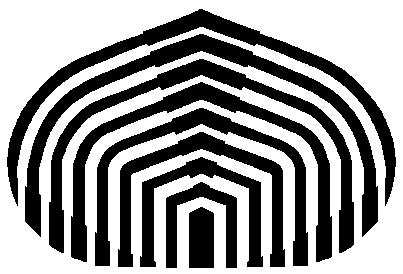
\includegraphics[height=80pt]{usb.jpg} \\
CI-5437 \\ Inteligencia Artificial I \\
Proyecto I\\
Búsqueda}
\author{Kelwin Fernández y Alejandro Machado\\
	Universidad Simón Bolívar} 
\date{Junio de 2010} 
\maketitle

\section{Decisiones de implementación}

\subsection{Representación de Perfiles}

Para la representación de un perfil, se optó por
compactar las preferencias que representen
la misma permutación de candidatos, de esta forma cada permutación
$a_0, a_1, \ldots, a_n$ de estos aparecerá a lo sumo una vez
en un perfil. En cada perfil, las preferencias se encuentran
almacenadas en un vector de forma ordenada.

Todo esto garantiza que cada perfil esté unívocamente representado
independientemente de cuáles cambios elementales han sido aplicados
para llegar
hasta él, evitando así la repetición de estados.

Se establece adicionalmente una relación de orden sobre perfiles,
$\sqsubseteq$, determinada por el orden lexicográfico de sus
preferencias.

\subsection{Representación de Estados}

Se tiene que en el espacio de búsqueda de este problema
el factor de ramificación (\emph{branching factor}) es de
lo sumo $m\cdot(n-1)$, donde $m$ es el número de electores y $n$
el número de candidatos.

Con el número máximo de candidatos establecido en
$250$ y suponiendo un (realista) número de $10^6$ de electores,
el factor de ramificación máximo será $249\times 10^6$.

Si la representación de cada estado tuviese la información
completa del perfil en ella, al ejecutar tan sólo un 
cambio elemental en el algoritmo de
búsqueda en amplitud habremos de mantener en memoria $55$
\textit{petabytes}.

Es por esto que se consideró 
optar por una representación compacta para los estados.

\subsubsection*{BFS}

En el caso de BFS el número de
nodos crecerá exponencialmente, por lo que una representación
compacta permitirá ahorrar recursos para que el algoritmo pueda
concluir su ejecución, en ciertos casos, sin agotar la memoria
del computador.

En lugar de almacenar un perfil completo, para cada estado
se guarda cuál fue el último cambio elemental realizado (cuál
candidato, en cuál preferencia), y un apuntador al estado padre.

Es necesario mantener una lista de estados ``cerrados" (ya
generados por el algoritmo) para una correcta implementación
de búsqueda en amplitud. En este caso, los estados visitados
se mantuvieron en un vector ordenado mediante la siguiente
relación de orden sobre Estado:

Sean $a, b$ estados generados por el algoritmo de búsqueda en
profundidad:

$$a \prec b \equiv f(a) < f(b) \ \vee \ (f(a) = f(b) \ \wedge \ Perfil(a) \sqsubseteq Perfil(b))$$

Donde $f$ es una función de clasificación asociada a los
estados y $Perfil(a)$ es el perfil generado por el estado
$a$. El valor de la función de clasificación para cada estado 
es precalculado al generarlo y se obtiene de forma semejante
a la función heurística heurística sugerida para el algoritmo
IDA*. Dando un orden $a_0, a_1, \ldots, a_n$ sobre los candidato,
tenemos que la función de clasificación de un estado $s$ viene
dada por:

$$\displaystyle f(s) = \sum_{i\in [0..n]} (B^i\cdot T'(a_i))\mbox{,}$$
    
\noindent donde $B$ es una constante que dispersa los
resultados de cada $T'(a_i)$ para evitar colisiones.
En esta implementación se escogió $B=10$, pues
este valor aportó resultados experimentales bastante satisfactorios.

La intuición detrás de esta decisión es la siguiente:
dos estados que evalúan a un diferente valor de la función de clasificación
deben ser distintos, y por lo tanto no hay que obtener los perfiles asociados
y compararlos, lo cual consume tiempo. En algunos casos, una búsqueda binaria
sobre el vector de nodos visitados puede arrojar el resultado que se necesita
sin tener que obtener ningún perfil.

Adicionalmente se almacena la profundidad de cada estado, a fin de no
seguir expandiendo fronteras del último nivel si ya se ha hallado una
solución en éste.

\subsubsection*{IDA*}

Para este algoritmo se utilizó un solo perfil. Cuando se va a expandir
un nodo, se considera uno de sus sucesores, se aplica un cambio elemental
y se llama recursivamente a su sucesor. Una vez que el sucesor devuelve
una respuesta, se desaplica el cambio elemental y se expande
al próximo hijo. Este proceso se repite hasta agotar los  cambios
elementales. 

De esta forma se reduce la memoria utilizada de $b\cdot d$ a $d$, donde
$b$ es el \textit{branching factor} y $d$ la longitud de camino. 

La lista de estados visitados se representa con un protocolo $LIFO$ que
permite simular las llamadas recursivas. En esta lista se presentan los
continuos cambios que se han venido aplicando para, de esta forma, poder
construir desde el estado inicial cada uno de los nodos intermedios.

\section{Obtención de sucesores}
\subsubsection*{BFS}
    Para obtener los sucesores de un estado, debe construirse primero
    el perfil asociado y luego aplicar todos los posibles cambios elementales
    sobre éste.

\subsubsection*{IDA*}
    Se aplica un cambio elemental sobre
    el perfil actual, y se explora el perfil hijo. Posteriormente,
    se deshace este cambio elemental; este proceso se repite para
   cada transición posible.

\section{Optimizaciones}

\subsubsection*{General}
    \begin{enumerate}
       \item Agregar un votante a una preferencia existente dentro de un perfil
       es $O(log(n))$, donde $n$ es el número de preferencias. Esto se logra
       manteniendo las preferencias ordenadas dentro de cada perfil.
    \end{enumerate}

\subsection*{BFS}
    \begin{enumerate}
       \item Los estados generados se mantienen en un vector ordenado,
       lo que garantiza, al utilizar búsqueda binaria, que a lo sumo
       se realizará un número logarítmico (en el número de estados
       generados) de comparaciones para determinar si se debe generar un
       nuevo estado.

		\item Se mantienen en memoria dos perfiles. Uno de ellos es el perfil
		correspondiente al estado recién expandido,
        y el otro corresponde al perfil padre de la iteración anterior. En
        búsqueda en profundidad, $b$ nodos
		de la frontera utilizarán el mismo padre, y con esto se evita
		el cálculo adicional de generar cada perfil desde el inicial.
		
		\item Se guarda el nivel de profundidad para no expandir nodos más
		allá de una meta.
		
		\item Gracias a la función de clasificación se evita generar
		cada perfil del vector de estados generados. 

		\item Los nodos generados se almacenan en un vector ordenados
		bajo la relación de orden dada para los estados, permitiendo
		así una búsqueda logarítmica.
\end{enumerate}

\subsection*{IDA*}

\begin{enumerate}
\item Al no verificar repeticiones sobre el espacio de búsqueda,
los tiempos de ejecución del algoritmo de IDA* mejoran considerablemente,
por lo tanto se consideró una opción adicional que permite correr el
algoritmo sin verificar repeticiones.

\end{enumerate}

\section{Opciones añadidas}

\begin{itemize}
\item \ms{-prop}: Imprime en cada intento de generar un nuevo estado
la proporción de comparaciones resueltas utilizando la función de
clasificación.

\item \ms{-nomem}: Permite ejecutar el algoritmo IDA* sin verificar

\end{itemize}

\section{Discusión de resultados}
En los siguientes ejemplos se evalúa el rendimiento
de la función de clasificación utilizada para
búsqueda en profundidad. Cada gráfico muestra la proporción
de nodos que no tuvieron que ser comparados
en corridas completas del algoritmo (nodos evitados entre nodos totales).
\pagebreak

\end{document}
